\documentclass[11pt,a4paper]{article}

\usepackage[utf8]{inputenc}
\usepackage[T1]{fontenc}
\usepackage[english]{babel}
\usepackage{lmodern}
\usepackage{amsmath,amssymb,amsfonts,amsthm}
\usepackage{mathtools}
\usepackage{bm}
\usepackage{graphicx}
\usepackage{booktabs}
\usepackage{enumitem}
\usepackage[margin=2.2cm]{geometry}
\usepackage{xcolor}
\usepackage[section]{placeins}
\usepackage[colorlinks=true,linkcolor=blue!60!black,citecolor=green!40!black,urlcolor=blue!60!black,bookmarksnumbered=true,bookmarksopen=true]{hyperref}
\usepackage[nameinlink]{cleveref}

\setlength{\parindent}{0pt}
\setlength{\parskip}{5pt}
\setlength{\emergencystretch}{3em}
\numberwithin{equation}{section}

\theoremstyle{remark}
\newtheorem*{remark}{Remark}

% ------------------------------------------------------------------ macros
\newcommand{\Om}{\hat{\Omega}}
\newcommand{\dd}{\mathrm{d}}
\newcommand{\kron}{\otimes}
\newcommand{\Lmax}{\Lambda}
\newcommand{\R}{\mathbb{R}}
\newcommand{\pderiv}[2]{\frac{\partial #1}{\partial #2}}
\newcommand{\pp}{{\bm{p}^{+}}}
\newcommand{\pmn}{{\bm{p}^{-}}}
\newcommand{\diag}{\operatorname{diag}}
\newcommand{\sgn}{\operatorname{sgn}}

\graphicspath{{images/}}

\title{Tensor-Train Methods for Neutron Transport}
\author{io}
\date{\today}

\begin{document}
\maketitle

\begin{abstract}
These notes collect the tensor-train (TT) tools and the discretization used to solve the time-dependent,
multigroup neutron transport equation in slab geometry (with full 3D angular dependence) as a single
all-at-once space--angle--energy--time linear system in TT format. The notation of
\cref{sec:tt-operator} follows the code \texttt{slab/tt\_neutron\_transport.py} (class \texttt{SlabTransportModel});
a dictionary between symbols and code variables is given in \cref{app:code}.
\end{abstract}

\tableofcontents
\newpage

%==========================================================================================
\section{Tensor-train toolbox}
\label{sec:tt}
%==========================================================================================

\subsection{TT tensors and TT operators}

A tensor-train (TT) decomposition of a $d$-dimensional tensor $\mathcal{A}\in\R^{n_1\times\dots\times n_d}$ is \cite{TT_Ose}
\begin{equation}
\mathcal{A}(i_1,\dots,i_d)=\sum_{\alpha_1=1}^{r_1}\cdots\sum_{\alpha_{d-1}=1}^{r_{d-1}}
G_1(1,i_1,\alpha_1)\,G_2(\alpha_1,i_2,\alpha_2)\cdots G_d(\alpha_{d-1},i_d,1),
\label{eq:tt}
\end{equation}
where $G_k\in\R^{r_{k-1}\times n_k\times r_k}$ ($r_0=r_d=1$) are the \emph{cores} (``wagons'') and $r_k$ the TT ranks.
With $n=\max_k n_k$ and $r=\max_k r_k$ the storage is $\mathcal{O}(dnr^2)$ instead of $\mathcal{O}(n^d)$.
A Kronecker (rank-one) product of vectors is the special case $r_1=\dots=r_{d-1}=1$.

A TT operator (TT matrix, TTM) $\mathcal{B}\in\R^{(m_1\cdots m_d)\times(n_1\cdots n_d)}$ is defined analogously with four-index cores,
\begin{equation}
\mathcal{B}(j_1,\dots,j_d;\,i_1,\dots,i_d)=\sum_{\beta_1,\dots,\beta_{d-1}}
W_1(1,j_1,i_1,\beta_1)\,W_2(\beta_1,j_2,i_2,\beta_2)\cdots W_d(\beta_{d-1},j_d,i_d,1),
\end{equation}
$W_k\in\R^{s_{k-1}\times m_k\times n_k\times s_k}$, storage $\mathcal{O}(dmns^2)$ instead of $\mathcal{O}(m^dn^d)$.
A Kronecker product $B_1\kron\dots\kron B_d$ is a TTM with all ranks one, and a sum of $R$ such products has ranks at most $R$.

Two facts are used repeatedly:
\begin{itemize}[nosep]
\item \textbf{Sums} of TT tensors add ranks; \textbf{matrix--vector products} multiply them ($r(\mathcal{B}\mathcal{X})\le s\,r$). In both cases the result is usually recompressed by \emph{TT rounding} (SVD-based, cost $\mathcal{O}(dnr^3)$) to a prescribed relative accuracy.
\item \textbf{Contraction} of one mode with a weight vector $w$, $\sum_{i_k}w_{i_k}G_k(\cdot,i_k,\cdot)$, yields an $r_{k-1}\times r_k$ matrix that can be absorbed into a neighbouring core, so that integrating out a variable costs $\mathcal{O}(n_kr^2)$ (function \texttt{integrate\_dim} in the code).
\end{itemize}

\subsection{AMEn linear solver}

AMEn (Alternating Minimal Energy) \cite{AMEn} solves $\mathcal{B}\mathcal{X}=\mathcal{F}$ with $\mathcal{B}$ a TTM and $\mathcal{F}$ a TT tensor, directly in TT format.
It sweeps through the cores of $\mathcal{X}$: at step $k$ all cores but $G_k$ are frozen (and orthogonalized), so that $\mathcal{X}=X_{\neq k}\,\mathrm{vec}(G_k)$ is linear in $G_k$ and the global system is projected onto a local one of size $r_{k-1}n_kr_k$,
\begin{equation}
X_{\neq k}^\top\mathcal{B}X_{\neq k}\,\mathrm{vec}(G_k)=X_{\neq k}^\top\mathcal{F}.
\end{equation}
For symmetric positive definite $\mathcal{B}$ this minimizes the energy functional over $G_k$; for the non-symmetric transport operator it is a Galerkin projection, which in practice works well but has no convergence guarantee.
After each local solve the core is \emph{enriched} with a low-rank (``\texttt{kickrank}'') approximation of the residual, which lets the TT ranks grow adaptively and gives a convergence rate comparable to steepest descent independently of the initial ranks.
Iterations stop when the local residuals are below the tolerance $\varepsilon$ or after \texttt{nswp} sweeps; local systems larger than \texttt{max\_full} are solved iteratively (GMRES) instead of directly.

\subsection{TT-cross approximation}

TT-cross \cite{TTcross} builds a TT approximation of a tensor from a small number of its entries, without ever forming it.
The cores are obtained by skeleton (CUR-type) interpolation on adaptively chosen index sets (fibres), selected with the \emph{maxvol} principle so that the interpolation submatrices are well conditioned.
The cost is $\mathcal{O}(dnr^2)$ function evaluations, which makes it the method of choice when the tensor is the discretization of a function that can be evaluated pointwise.

\paragraph{Example: high-dimensional quadrature.}
Discretize $f(x_1,\dots,x_d)$ on a tensor grid with $n$ nodes and weights $w^{(k)}_{i}$ per dimension:
\begin{equation}
I=\int f(x_1,\dots,x_d)\,\dd x_1\cdots\dd x_d\approx\sum_{i_1=1}^{n}\cdots\sum_{i_d=1}^{n}F(i_1,\dots,i_d)\,w^{(1)}_{i_1}\cdots w^{(d)}_{i_d}.
\end{equation}
In full format this costs $\mathcal{O}(n^d)$ storage and operations. If $F$ is approximated by TT-cross, the sum factorizes into a product of small matrices,
\begin{equation}
I\approx\prod_{k=1}^{d}\Big(\sum_{i_k=1}^{n}w^{(k)}_{i_k}\,G_k(\cdot,i_k,\cdot)\Big),
\end{equation}
computed left to right at cost $\mathcal{O}(dnr^2)$.
For $d=10$, $n=100$ the full tensor has $10^{20}$ entries ($\approx8\times10^{8}$\,TB in double precision, $\approx10^{8}$\,s $\approx3$ years at $1$\,TFLOP/s just to sum it), whereas the TT computation took $0.3$\,s and $28$\,kB of memory.

\paragraph{Example: high-dimensional convolution.}
Consider
\begin{equation}
h(x)=\int g(x-y)\,f(y)\,\dd y,\qquad x,y\in\R^d,
\end{equation}
discretized as
\begin{equation}
H(x_1,\dots,x_d)\approx\sum_{y_1,\dots,y_d}\mathsf{G}(x_1,\dots,x_d,y_1,\dots,y_d)\,F(y_1,\dots,y_d)\,w(y_1)\cdots w(y_d),
\qquad \mathsf{G}(x,y)=g(x-y).
\end{equation}
Store $F$ as a $d$-dimensional TT with ranks $\beta$ and the kernel $\mathsf{G}$ as a $2d$-dimensional TT (variables ordered $x_1,\dots,x_d,y_1,\dots,y_d$) with ranks $\alpha$, both obtained by TT-cross:
\begin{equation}
\mathsf{G}=G^{(1)}(1,x_1,\alpha_1)\cdots G^{(d)}(\alpha_{d-1},x_d,\alpha_d)\;G^{(d+1)}(\alpha_d,y_1,\alpha_{d+1})\cdots G^{(2d)}(\alpha_{2d-1},y_d,1),
\end{equation}
summation over repeated rank indices implied. For $j=1,\dots,d$ contract the $y_j$ modes,
\begin{equation}
T^{(j)}(\alpha_{d+j-1},\alpha_{d+j},\beta_{j-1},\beta_j)=\sum_{y_j}G^{(d+j)}(\alpha_{d+j-1},y_j,\alpha_{d+j})\,F^{(j)}(\beta_{j-1},y_j,\beta_j)\,w(y_j),
\end{equation}
and eliminate them from right to left, with $\alpha_{2d}=\beta_d=1$:
\begin{gather}
A^{(d)}(\alpha_{2d-1},\beta_{d-1})=T^{(d)}(\alpha_{2d-1},1,\beta_{d-1},1),\\
A^{(j)}(\alpha_{d+j-1},\beta_{j-1})=\sum_{\alpha_{d+j},\beta_j}T^{(j)}(\alpha_{d+j-1},\alpha_{d+j},\beta_{j-1},\beta_j)\,A^{(j+1)}(\alpha_{d+j},\beta_j),\quad j=d-1,\dots,1.
\end{gather}
Since $\beta_0=1$, $A^{(1)}$ is a vector of length $r_d=\alpha_d$ and
\begin{equation}
H(x_1,\dots,x_d)=G^{(1)}(1,x_1,\alpha_1)\cdots G^{(d)}(\alpha_{d-1},x_d,\alpha_d)\,A^{(1)}(\alpha_d).
\end{equation}
The result has the ranks of the $x$-half of the kernel, and the cost is $\mathcal{O}(dn\alpha^2\beta^2)$.
Treating $\mathsf{G}$ as a TT matrix and computing a matrix--vector product would instead create an intermediate with ranks $\alpha\beta$, whose rounding costs $\mathcal{O}(dn\alpha^3\beta^3)$.

%==========================================================================================
\section{Model problem}
\label{sec:model}
%==========================================================================================

\subsection{Multigroup time-dependent transport in a slab}

In a homogeneous slab $z\in[0,L]$, with full 3D angular dependence, the multigroup (MG) transport equation for the angular flux $\psi_g(z,\Om,t)$ is
\begin{equation}
\begin{cases}
\left(\dfrac{1}{v_g}\dfrac{\partial}{\partial t}+\mu\dfrac{\partial}{\partial z}+\sigma_{t,g}\right)\psi_g
=\displaystyle\sum_{g'=1}^{G}\int_{4\pi}\sigma_{s,g'\to g}(\Om\cdot\Om')\,\psi_{g'}(z,\Om',t)\,\dd\Om'+Q_g(z,\Om,t),\\[3mm]
\psi_g(0,\Om,t)=\psi^{\mathrm{left}}_{g}(\Om,t), \qquad \mu>0,\\[1mm]
\psi_g(L,\Om,t)=\psi^{\mathrm{right}}_{g}(\Om,t), \qquad \mu<0,\\[1mm]
\psi_g(z,\Om,0)=\psi^{\mathrm{init}}_{g}(z,\Om),
\end{cases}
\label{eq:MGNTE}
\end{equation}
with $\Om=\Om(\mu,\varphi)$, $\mu=\Om\cdot\hat z=\cos\theta$, $g=1$ the fastest group.

The full $(\mu,\varphi)$ dependence is kept so that the TT structure of the scattering kernel on $\mathbb{S}^2$ can be reused in 3D. The slab is invariant under rotations about $\hat z$, so the solution is azimuthally symmetric whenever $\psi^{\mathrm{left}}_g,\psi^{\mathrm{right}}_g,\psi^{\mathrm{init}}_g,Q_g$ are.

\subsection{Scattering kernel in spherical harmonics}
\label{sec:kernel}

Expand the kernel in Legendre polynomials,
\begin{equation}
\sigma_{s,g'\to g}(\mu_0)=\sum_{l=0}^{\Lmax}\frac{2l+1}{4\pi}\,\sigma^{l}_{s,g'\to g}\,P_l(\mu_0),\qquad\mu_0=\Om\cdot\Om',
\end{equation}
and use the addition theorem $P_l(\Om\cdot\Om')=\frac{4\pi}{2l+1}\sum_{m=-l}^{l}Y_{lm}(\Om)Y_{lm}(\Om')$ with the \emph{real} orthonormal spherical harmonics
\begin{equation}
Y_{lm}(\Om)=A_{lm}(\mu)\,\Pi_m(\varphi),\qquad
A_{lm}(\mu)=\sqrt{\frac{2l+1}{4\pi}\frac{(l-|m|)!}{(l+|m|)!}}\;P_l^{|m|}(\mu),
\end{equation}
\begin{equation}
\Pi_m(\varphi)=\begin{cases}\sqrt2\cos(m\varphi) & m>0,\\ 1 & m=0,\\ \sqrt2\sin(|m|\varphi) & m<0,\end{cases}
\label{eq:Ylm}
\end{equation}
($\int_{4\pi}Y_{lm}Y_{l'm'}\,\dd\Om=\delta_{ll'}\delta_{mm'}$; the Condon--Shortley phase is irrelevant since $A_{lm}$ always appears squared). Then
\begin{equation}
\sigma_{s,g'\to g}(\Om\cdot\Om')=\sum_{l=0}^{\Lmax}\sigma^{l}_{s,g'\to g}\sum_{m=-l}^{l}Y_{lm}(\Om)\,Y_{lm}(\Om'),
\label{eq:kernel-Ylm}
\end{equation}
i.e.\ $Y_{lm}$ are eigenfunctions of the angular scattering operator. Energy enters only through $\sigma^{l}_{s,g'\to g}$ (independent of $m$ by isotropy of the medium).

\subsection{Toy model: Henyey--Greenstein kernel and a moderator-like group structure}
\label{sec:toy}

All lengths are in mean free paths, $\sigma_{t,g}=1$, so interaction coefficients are probabilities per collision. The kernel factorizes into energy and angle,
\begin{equation}
\sigma_{s,g'\to g}(\Om'\cdot\Om)=c_{gg'}\,K_s(\Om'\cdot\Om),\qquad \int_{4\pi}K_s\,\dd\Om=1,
\end{equation}
with $c_{gg'}$ the probability that a collision in group $g'$ scatters the neutron into group $g$.

\paragraph{Angular kernel.}
The Henyey--Greenstein (HG) phase function \cite{HenyeyGreenstein1941}
\begin{equation}
K_s(\mu_0)=\frac{1}{4\pi}\frac{1-\gamma^2}{(1+\gamma^2-2\gamma\mu_0)^{3/2}}
=\sum_{l=0}^{\infty}\frac{2l+1}{4\pi}\gamma^l P_l(\mu_0)
=\sum_{l=0}^{\infty}\gamma^l\sum_{m=-l}^{l}Y_{lm}(\Om)Y_{lm}(\Om'),\qquad\gamma\in[0,1),
\end{equation}
interpolates between isotropic ($\gamma=0$) and strongly forward-peaked ($\gamma\to1$) scattering. Truncation at $l=\Lmax$ preserves normalization (the $l=0$ term is untouched); since $|P_l|\le1$ the pointwise truncation error is bounded by $\sum_{l>\Lmax}\frac{2l+1}{4\pi}\gamma^l=\mathcal{O}(\Lmax\gamma^{\Lmax+1})$.

\paragraph{Energy structure.}
Group edges are logarithmically spaced in $[E_{\min},E_{\max}]$ and ordered decreasingly; $E_g$ is the geometric centre of group $g$, so $g+1$ is the next slower group. Velocities and absorption follow
\begin{equation}
v_g=v_0\sqrt{E_g/E_{\max}},\qquad \sigma_{a,g}=\sigma_{a,0}\,\frac{v_0}{v_g}\quad(1/v\text{ law}).
\end{equation}
$\sigma_{a,g}$ is largest in the slowest group, so $\sigma_{a,g}\le1\ \forall g\iff\sigma_{a,0}\le v_G/v_0$. The code fixes the absorption probability $s_a\in[0,1]$ of the slowest group, $\sigma_{a,0}=s_a v_G/v_0$.

Scattering is either in-group or into the next lower group, with a down-scatter fraction $\eta\in[0,1]$:
\begin{equation}
c_{gg'}=(1-\eta)(1-\sigma_{a,g'})\,\delta_{gg'}+\eta\,(1-\sigma_{a,g'})\,\delta_{g,g'+1},\qquad g'<G,
\end{equation}
and $c_{GG}=1-\sigma_{a,G}$ (no down-scatter out of the last group; otherwise the neutron would leave the energy range and count as an extra removal). Thus $\sum_g c_{gg'}=1-\sigma_{a,g'}$: what is not scattered is absorbed, and $C=[c_{gg'}]$ is lower bidiagonal.

Comparing with \eqref{eq:kernel-Ylm}, $\sigma^l_{s,g'\to g}=\gamma^l c_{gg'}$: \emph{the energy factor is the same matrix $C$ for every $(l,m)$}, which is what makes the scattering operator rank one across the angle--energy bond (\cref{sec:tt-operator}).

%==========================================================================================
\section{Discretization}
\label{sec:discr}
%==========================================================================================

\paragraph{Index conventions.}
\begin{center}
\begin{tabular}{@{}lll@{}}
\toprule
Index & Range & Meaning \\
\midrule
$i,i'$ & $1,\dots,N_z$ & spatial cells \\
$a,b$ & $0,\dots,p$ & Legendre modes within a cell \\
$n,n'$ & $1,\dots,N_\mu$ & polar ordinates $\mu_n$ \\
$q,q'$ & $1,\dots,N_\varphi$ & azimuthal ordinates $\varphi_q$ \\
$g,g'$ & $1,\dots,G$ & energy groups \\
$k,k'$ & $1,\dots,N_t$ & time steps \\
$l$ & $0,\dots,\Lmax$ & degree of the scattering expansion \\
$m$ & $-l,\dots,l$ & order of the real spherical harmonics \\
\bottomrule
\end{tabular}
\end{center}
Unprimed indices label equations (rows), primed ones unknowns (columns).

\subsection{Angle: discrete ordinates}
\label{sec:angle}

The $S_N$ method uses the product set $\Om_{nq}=\Om(\mu_n,\varphi_q)$ with
\begin{itemize}[nosep]
\item $\mu_n,w_n$: $N_\mu$-point Gauss--Legendre rule on $[-1,1]$ ($\sum_nw_n=2$). For even $N_\mu$ no ordinate has $\mu_n=0$, so the upwind choice below is unambiguous.\footnote{For odd $N_\mu$ (e.g.\ $N_\mu=3$ in \cref{sec:absorber}) the ordinate $\mu=0$ has no streaming at all and reduces to an ODE in time; the code handles it consistently since $\mu^\pm=0$ there.}
\item $\varphi_q=2\pi(q-1)/N_\varphi$, $w_q=2\pi/N_\varphi$: trapezoidal rule, exact for trigonometric polynomials of degree $<N_\varphi$.
\end{itemize}
Hence $\int_{4\pi}f\,\dd\Om\approx\sum_{n,q}w_nw_q\,f(\Om_{nq})$. Products $Y_{lm}Y_{l'm'}$ with $l,l'\le\Lmax$ are polynomials of degree $\le2\Lmax$ in $\mu$ (when $m=m'$) and trigonometric polynomials of degree $\le2\Lmax$ in $\varphi$, so the spherical harmonics are \emph{discretely} orthonormal, and the discrete kernel has exactly the eigenpairs $Y_{lm}\mapsto\sigma^l Y_{lm}$, provided
\begin{equation}
N_\mu\ge\Lmax+1,\qquad N_\varphi\ge2\Lmax+1.
\label{eq:quad-exact}
\end{equation}
Write $\mu^+_n=\max(\mu_n,0)$ and $\mu^-_n=\min(\mu_n,0)$, so $\mu_n=\mu_n^++\mu_n^-$.

\subsection{Space: discontinuous Galerkin}
\label{sec:dg}

Uniform mesh $K_i=[z_{i-1/2},z_{i+1/2}]$, $h=L/N_z$, local coordinate $z=z_i+\tfrac h2\xi$, $\xi\in[-1,1]$. In each cell
\begin{equation}
\psi_g(z,\Om_{nq},t)\approx\sum_{b=0}^{p}\psi^{nq}_{g,ib}(t)\,P_b(\xi),\qquad z\in K_i,
\end{equation}
and we collect the modes in $\bm\psi_i=(\psi_{i0},\dots,\psi_{ip})^\top\in\R^{p+1}$ (indices $n,q,g$ dropped when not needed).
Cross sections are piecewise constant. Testing with $P_a$ over $K_i$ only requires three local objects:
\begin{gather}
M_h=\diag\Big(\frac{h}{2a+1}\Big)_{a=0}^{p},\qquad
S_{ab}=\int_{-1}^{1}P_b\,P_a'\,\dd\xi=\begin{cases}2 & a>b,\ a+b\text{ odd},\\0&\text{otherwise,}\end{cases}\\
\pp=\big(P_a(1)\big)_a=\bm 1,\quad \pmn=\big(P_a(-1)\big)_a=\big((-1)^a\big)_a .
\end{gather}
$M_h$ is the local mass matrix ($\int_{K_i}P_aP_b\,\dd z=\frac h2\frac{2}{2a+1}\delta_{ab}$) and $S$ follows from $P_a'=\sum_{b<a,\,a+b\text{ odd}}(2b+1)P_b$.

\paragraph{Streaming.} Since $\dd z\,\partial_z=\dd\xi\,\partial_\xi$, integration by parts gives
\begin{equation}
\int_{K_i}\mu_n\,\partial_z\psi\,P_a\,\dd z=\mu_n\big[P_a(1)\,\psi^*_{i+1/2}-P_a(-1)\,\psi^*_{i-1/2}\big]-\mu_n\,(S\bm\psi_i)_a ,
\end{equation}
with upwind traces $\psi^*_{i+1/2}=\pp\cdot\bm\psi_i$, $\psi^*_{i-1/2}=\pp\cdot\bm\psi_{i-1}$ for $\mu_n>0$ and $\psi^*_{i+1/2}=\pmn\cdot\bm\psi_{i+1}$, $\psi^*_{i-1/2}=\pmn\cdot\bm\psi_i$ for $\mu_n<0$. In vector form
\begin{equation}
\mu_n^+\big(\pp\pp^{\!\top}\bm\psi_i-\pmn\pp^{\!\top}\bm\psi_{i-1}\big)
+\mu_n^-\big(\pp\pmn^{\!\top}\bm\psi_{i+1}-\pmn\pmn^{\!\top}\bm\psi_i\big)
-\mu_n\,S\bm\psi_i .
\label{eq:streaming-local}
\end{equation}
Information flows along the direction of flight: cell $i$ couples to $i-1$ for $\mu>0$ and to $i+1$ for $\mu<0$.

\paragraph{Boundary conditions.}
For $i=1$, $\mu_n>0$ the trace $\psi^*_{1/2}=\psi^{\mathrm{left}}$ is known, and the term $-\mu_nP_a(-1)\psi^{\mathrm{left}}$ moves to the right-hand side; likewise for $i=N_z$, $\mu_n<0$, the term $+\mu_nP_a(1)\psi^{\mathrm{right}}$:
\begin{equation}
\bm f^{\,\mathrm{left}}=\mu_n^+\,\psi^{\mathrm{left}}_g(\Om_{nq},t)\,\pmn\ \ \text{(cell 1)},\qquad
\bm f^{\,\mathrm{right}}=-\mu_n^-\,\psi^{\mathrm{right}}_g(\Om_{nq},t)\,\pp\ \ \text{(cell $N_z$)},
\label{eq:bc}
\end{equation}
both non-negative weights since $-\mu^-_n=|\mu_n|$ for $\mu_n<0$. The neighbour terms in \eqref{eq:streaming-local} are dropped at the boundary cells.

\paragraph{Semi-discrete system.}
For cell $i$, group $g$, direction $\Om_{nq}$:
\begin{multline}
\frac{1}{v_g}M_h\dot{\bm\psi}^{nq}_{g,i}
+\mu_n^+\big(\pp\pp^{\!\top}\bm\psi^{nq}_{g,i}-\pmn\pp^{\!\top}\bm\psi^{nq}_{g,i-1}\big)
+\mu_n^-\big(\pp\pmn^{\!\top}\bm\psi^{nq}_{g,i+1}-\pmn\pmn^{\!\top}\bm\psi^{nq}_{g,i}\big)
-\mu_nS\bm\psi^{nq}_{g,i}
+\sigma_{t,g}M_h\bm\psi^{nq}_{g,i}\\
=\sum_{g'}\sum_{n',q'}w_{n'}w_{q'}\,\sigma_{s,g'\to g}(\Om_{nq}\cdot\Om_{n'q'})\,M_h\bm\psi^{n'q'}_{g',i}
+\bm Q^{nq}_{g,i}(t)+\delta_{i1}\bm f^{\,\mathrm{left}}+\delta_{iN_z}\bm f^{\,\mathrm{right}},
\label{eq:semidiscrete}
\end{multline}
where $(\bm Q^{nq}_{g,i})_a=\int_{K_i}Q_g(z,\Om_{nq},t)P_a\,\dd z$ is the projected source (equal to $M_h$ times its Legendre coefficients).

\subsection{Time: backward Euler, all at once}
\label{sec:time}

Uniform steps $t_k=k\Delta t$, $k=1,\dots,N_t$, $\Delta t=T/N_t$, unknowns $\bm\psi^k=\bm\psi(t_k)$. Backward Euler evaluates every term at $t_k$ and replaces $\dot{\bm\psi}(t_k)$ by $(\bm\psi^k-\bm\psi^{k-1})/\Delta t$.
Instead of stepping, all $N_t$ steps are solved simultaneously: the coupling $-\bm\psi^{k-1}/\Delta t$ becomes a sub-diagonal in the time index, and for $k=1$ the known $\bm\psi^0$ moves to the right-hand side,
\begin{equation}
\bm f^{\,\mathrm{init}}=\frac{\delta_{k1}}{v_g\Delta t}\,\Big(\int_{K_i}\psi^{\mathrm{init}}_g(z,\Om_{nq})P_a\,\dd z\Big)_a .
\end{equation}
The scheme is first order in $\Delta t$ and (for smooth solutions) of order $p+1$ in $h$.

%==========================================================================================
\section{All-at-once tensor-train formulation}
\label{sec:tt-operator}
%==========================================================================================

\subsection{Unknown and building blocks}

The discrete unknown is a 5-dimensional tensor, stored as a TT with cores ordered as in the code,
\begin{equation}
\Psi(s,n,q,g,k)=G^{(1)}(s,r_1)\,G^{(2)}(r_1,n,r_2)\,G^{(3)}(r_2,q,r_3)\,G^{(4)}(r_3,g,r_4)\,G^{(5)}(r_4,k),
\qquad s=(i,a),
\end{equation}
where $s$ is the composite cell/mode index of size $N_s=N_z(p+1)$ (mode index fastest). All operators below are Kronecker products in the order $s\kron n\kron q\kron g\kron k$; identities are written $I$ with the size implied by their slot. Only the following factors are needed.

\begin{center}\small
\renewcommand{\arraystretch}{1.35}
\begin{tabular}{@{}lll@{}}
\toprule
Slot & Factor & Definition \\
\midrule
space $s$ & $M$ & $I_{N_z}\kron M_h$ \hfill (mass) \\
 & $\mathsf{S}$ & $I_{N_z}\kron S$ \hfill (volume streaming) \\
 & $U^{+}$ & $I_{N_z}\kron\pp\pp^{\!\top}-E^{-}\kron\pmn\pp^{\!\top}$ \hfill (faces, $\mu>0$) \\
 & $U^{-}$ & $E^{+}\kron\pp\pmn^{\!\top}-I_{N_z}\kron\pmn\pmn^{\!\top}$ \hfill (faces, $\mu<0$) \\
angle $n,q$ & $D_\mu,\ D_\mu^{\pm}$ & $\diag(\mu_n)$, $\diag(\mu_n^\pm)$ \\
 & $K$ & discrete HG kernel, 2-core TTM over $(n,q)$, \cref{eq:K} \\
energy $g$ & $V,\ \Sigma_t$ & $\diag(v_g)$, $\diag(\sigma_{t,g})$ \\
 & $C$ & group transfer matrix $[c_{gg'}]$, \cref{sec:toy} \\
time $k$ & $D_t$ & $\Delta t^{-1}(I-E^-)$ \hfill (backward difference) \\
\bottomrule
\end{tabular}
\end{center}
Here $E^-$ and $E^+$ are the lower and upper shift matrices, $(E^-)_{ii'}=\delta_{i',i-1}$, $(E^+)_{ii'}=\delta_{i',i+1}$ (used both for cells and time steps).

\paragraph{Discrete scattering kernel.}
For HG scattering the angular part of $\sum_{n'q'}w_{n'}w_{q'}\sigma_s(\Om_{nq}\cdot\Om_{n'q'})(\cdot)$ is the matrix
\begin{equation}
\begin{aligned}
K_{(nq),(n'q')}&=\sum_{l=0}^{\Lmax}\gamma^l\sum_{m=-l}^{l}Y_{lm}(\Om_{nq})\,Y_{lm}(\Om_{n'q'})\,w_{n'}w_{q'},\\
K&=\sum_{m=-\Lmax}^{\Lmax}\underbrace{\Big[\sum_{l=|m|}^{\Lmax}\gamma^l\,\bm a_{lm}\bm a_{lm}^{\!\top}W_\mu\Big]}_{\mu\text{ core}}\kron\underbrace{\big[\bm\pi_m\bm\pi_m^{\!\top}W_\varphi\big]}_{\varphi\text{ core}},
\end{aligned}
\label{eq:K}
\end{equation}
with $\bm a_{lm}=(A_{lm}(\mu_n))_n$, $\bm\pi_m=(\Pi_m(\varphi_q))_q$, $W_\mu=\diag(w_n)$, $W_\varphi=\diag(w_q)$.
The code (\texttt{heneey\_greenstein}) sums the $(\Lmax+1)^2$ rank-one terms and rounds; grouping by $m$ as in \eqref{eq:K} shows that the exact rank of $K$ across the $\mu|\varphi$ bond is at most $2\Lmax+1$ (and $1$ for azimuthally symmetric problems, where only $m=0$ contributes and one may take $N_\varphi=1$).

\subsection{Operator}

Writing each term of \eqref{eq:semidiscrete}, for all time steps at once, as a Kronecker product gives the all-at-once system $\mathcal{A}\Psi=F$ with
\begin{equation}
\boxed{
\begin{aligned}
\mathcal{A}={}&M\kron I\kron I\kron V^{-1}\kron D_t
&&\text{time derivative}\\
&+M\kron I\kron I\kron\Sigma_t\kron I
&&\text{collision}\\
&-\mathsf{S}\kron D_\mu\kron I\kron I\kron I
&&\text{streaming, volume}\\
&+U^{+}\kron D_\mu^{+}\kron I\kron I\kron I
+U^{-}\kron D_\mu^{-}\kron I\kron I\kron I
&&\text{streaming, faces (upwind)}\\
&-M\kron K\kron C\kron I
&&\text{scattering}
\end{aligned}}
\label{eq:A}
\end{equation}
which is literally \texttt{construct\_tt\_operator}. Each line is a rank-one TTM except the scattering term, whose $\mu|\varphi$ rank is that of $K$; before rounding the sum has TT rank at most $6$ across every bond except $\mu|\varphi$, where it is at most $5+r_K$.

\paragraph{General scattering.} For a kernel whose Legendre moments $\Sigma^l=[\sigma^l_{s,g'\to g}]$ are not proportional to a single matrix, the last line becomes $-\sum_{l,m}M\kron\big(\bm a_{lm}\bm a_{lm}^{\!\top}W_\mu\big)\kron\big(\bm\pi_m\bm\pi_m^{\!\top}W_\varphi\big)\kron\Sigma^l\kron I$, a sum of $(\Lmax+1)^2$ rank-one TTMs whose angle--energy rank is at most $\Lmax+1$.

\begin{remark}[decoupling in $m$]
All terms except scattering are diagonal in $\varphi_q$, and the scattering is diagonal in $m$ after the change of basis $\varphi_q\mapsto\Pi_m$. Hence the system is block diagonal in $m$; for azimuthally symmetric data only $m=0$ is populated.
\end{remark}

\subsection{Right-hand side}

$F=F_Q+F_{\mathrm{init}}+F_{\mathrm{left}}+F_{\mathrm{right}}$ (\texttt{construct\_tt\_rhs}), each built as a Kronecker product when the data are separable, or as a sum of such products otherwise:
\begin{align}
F_Q&=\bm Q_z\kron\bm Q_\mu\kron\bm Q_\varphi\kron\bm Q_E\kron\bm Q_t, & (\bm Q_z)_{(i,a)}&=\int_{K_i}Q_z(z)P_a\,\dd z,\\
F_{\mathrm{init}}&=\tfrac{1}{\Delta t}\,\bm\Psi^0_z\kron\bm\Psi^0_\mu\kron\bm\Psi^0_\varphi\kron V^{-1}\bm\Psi^0_E\kron\bm e_1, & (\bm\Psi^0_z)_{(i,a)}&=\int_{K_i}\psi^{\mathrm{init}}_z(z)P_a\,\dd z,\\
F_{\mathrm{left}}&=(\bm e_1\kron\pmn)\kron D_\mu^{+}\bm b^{L}_\mu\kron\bm b^L_\varphi\kron\bm b^L_E\kron\bm b^L_t, \\
F_{\mathrm{right}}&=-(\bm e_{N_z}\kron\pp)\kron D_\mu^{-}\bm b^{R}_\mu\kron\bm b^R_\varphi\kron\bm b^R_E\kron\bm b^R_t,
\end{align}
where subscripts denote the separable factors of the data evaluated on the grids (e.g.\ $Q_g(z,\Om,t)=Q_z(z)Q_\mu(\mu)Q_\varphi(\varphi)(\bm Q_E)_gQ_t(t)$), $\bm e_j$ is the $j$-th unit vector, and $D_\mu^\pm$ implement the restriction to incoming directions in \eqref{eq:bc}.

\subsection{Post-processing}

The solution is returned as modal coefficients. Point values are obtained by contracting the space core with the Legendre basis at $N_{\mathrm{rec}}$ Gauss points per cell (\texttt{legendre\_to\_physical\_space}); the scalar flux $\phi_g(z,t)=\sum_{n,q}w_nw_q\psi_g(z,\Om_{nq},t)$ is computed by contracting the $\varphi$ and $\mu$ cores with their weights, without leaving the TT format.

%==========================================================================================
\section{Verification}
\label{sec:verification}
%==========================================================================================

\subsection{Convergence study with a manufactured solution}
\label{sec:mms}

Take the HG/moderator model of \cref{sec:toy} with the manufactured solution
\begin{equation}
\psi_g(z,\Om,t)=\alpha_g\,f(z)\,Y(\Om)\,e^{-t/\tau},\qquad
f(z)=a_1\sin\frac{\pi z}{L}+a_2\cos\frac{\pi z}{L},\qquad
Y=b_0Y_{00}+b_1Y_{11}+b_2Y_{2,-1},
\end{equation}
where $\alpha_g$ are arbitrary group amplitudes (\texttt{amp\_g} in the code; not the group energies). The solution is smooth, rank one across every bond except $\mu|\varphi$, where it has rank three (one per spherical harmonic, as the $\Pi_m$ are distinct). Since $Y_{lm}$ is mapped to $\gamma^lY_{lm}$ by the HG kernel (exactly, if $\Lmax\ge2$ and \eqref{eq:quad-exact} holds for the modes involved), substitution into \eqref{eq:MGNTE} gives the source
\begin{gather}
Q_g=\Big[\Big(\sigma_{t,g}-\frac{1}{\tau v_g}\Big)\alpha_g\,f(z)\,Y(\Om)
+\alpha_g\,f'(z)\,\mu\,Y(\Om)
-(C\bm\alpha)_g\,f(z)\,Y_\gamma(\Om)\Big]e^{-t/\tau},\\
Y_\gamma=b_0Y_{00}+\gamma b_1Y_{11}+\gamma^2b_2Y_{2,-1},
\end{gather}
with $f'(z)=\frac{\pi}{L}\big(a_1\cos\frac{\pi z}{L}-a_2\sin\frac{\pi z}{L}\big)$ and $(C\bm\alpha)_g=\sum_{g'}c_{gg'}\alpha_{g'}$. Initial and inflow data are the restrictions of the exact solution:
\begin{equation}
\psi^{\mathrm{init}}_g=\alpha_gf(z)Y(\Om),\qquad
\psi^{\mathrm{left}}_g=a_2\,\alpha_gY(\Om)e^{-t/\tau}\ (\mu>0),\qquad
\psi^{\mathrm{right}}_g=-a_2\,\alpha_gY(\Om)e^{-t/\tau}\ (\mu<0).
\end{equation}
Every term of $Q_g$ is separable, so $F$ is a short sum of rank-one TTs. The error is the relative Frobenius norm at the reconstruction points, over all ordinates, groups and time steps, computed in TT format:
\begin{equation}
e=\frac{\|\Psi-\Psi_{\mathrm{exact}}\|_F}{\|\Psi_{\mathrm{exact}}\|_F}.
\end{equation}
Two sweeps isolate the two error sources:
\begin{itemize}[nosep]
\item \emph{space}: $N_z$ varies at $N_t=512$, and the time derivative in $Q_g$ is replaced by the exact backward difference $(e^{-t_k/\tau}-e^{-t_{k-1}/\tau})/\Delta t$, so that backward Euler is exact in time and the rate $h^{p+1}$ is visible;
\item \emph{time}: $N_t$ varies at $N_z=512$ with the analytic derivative, showing the rate $\Delta t$.
\end{itemize}

\begin{figure}[h!]
\centering
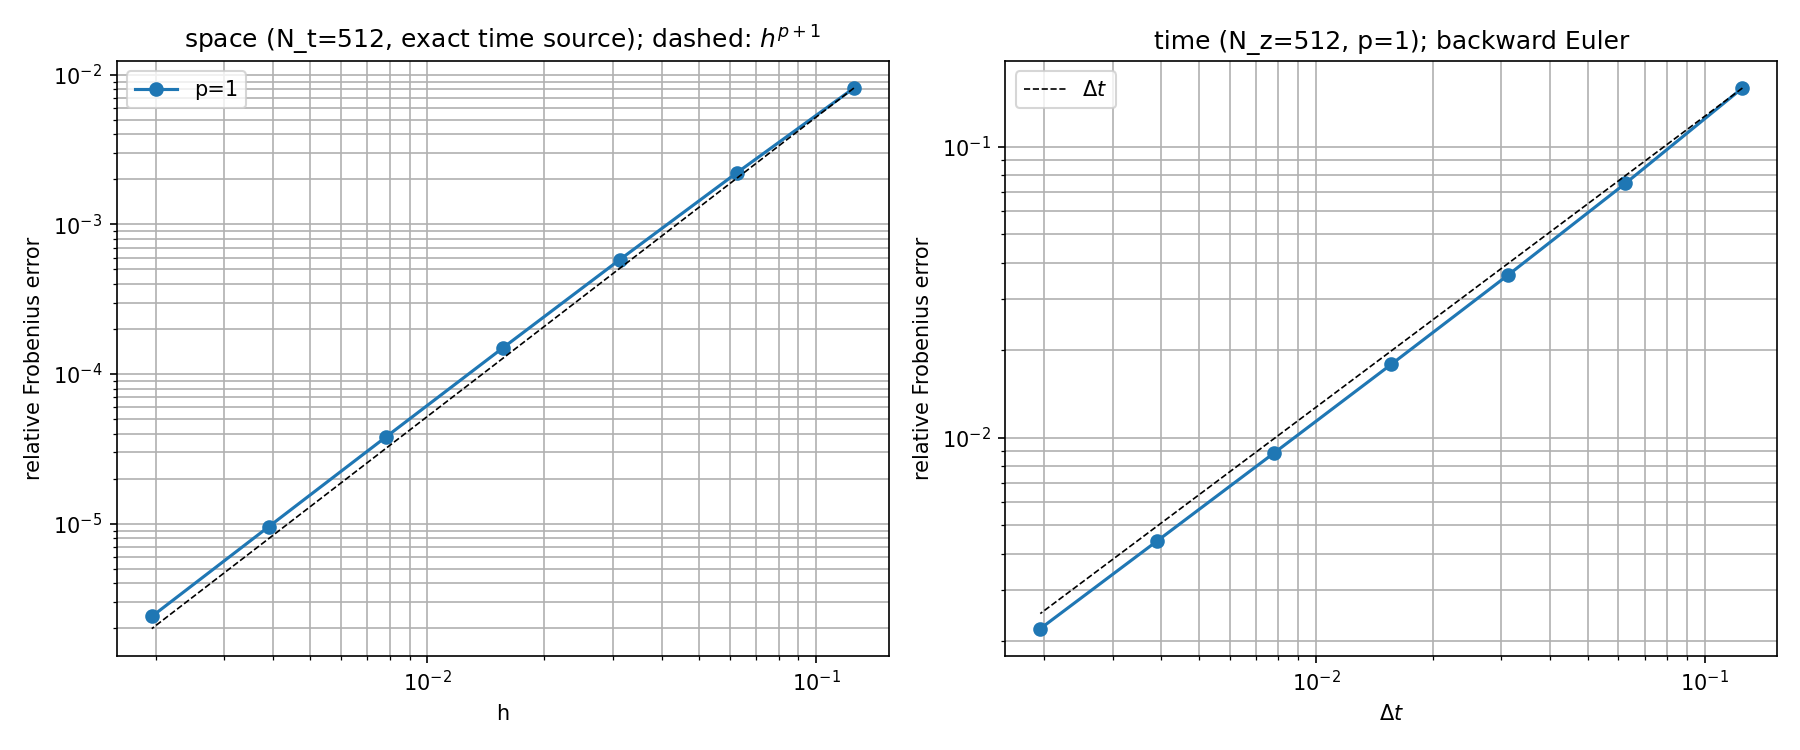
\includegraphics[width=\textwidth]{convergence_manuf_sol.png}
\caption{Manufactured-solution convergence. Left: space sweep ($N_t=512$, exact backward-difference time source, $p=1$), dashed line $h^{p+1}$. Right: time sweep ($N_z=512$, $p=1$), dashed line $\Delta t$. $N_\mu=N_\varphi=8$, $G=2$, $\gamma=0.5$, $\Lmax=4$, $L=T=1$; AMEn $\varepsilon=10^{-10}$, 15 sweeps, kickrank 2. Both sweeps show the expected orders.}
\label{fig:convergence}
\end{figure}

\FloatBarrier
\subsection{Purely absorbing medium}
\label{sec:absorber}

Without scattering \eqref{eq:MGNTE} reduces to
\begin{equation}
\left(\frac{1}{v_g}\pderiv{}{t}+\mu\pderiv{}{z}+\sigma_{t,g}\right)\psi_g=Q_g,
\end{equation}
groups and directions decouple, and each $(g,\Om)$ is an advection--reaction problem solvable by characteristics \cite{HandbookTransport}.

\paragraph{Characteristics.}
For fixed $(g,\Om)$, the characteristic through $(z,t)$, parametrized backwards by the path length $s\ge0$, is $z'=z-\mu s$, $t'=t-s/v_g$. Along it
\begin{equation}
\frac{\dd}{\dd s}\psi_g(z-\mu s,\Om,t-s/v_g)=-\Big(\frac{1}{v_g}\partial_t+\mu\partial_z\Big)\psi_g=\sigma_{t,g}\psi_g-Q_g .
\end{equation}
Going backwards the characteristic leaves the domain either through $t'=0$ (it carries the initial condition) or through the inflow boundary (it carries the boundary data), whichever comes first. The time of flight from the inflow boundary is
\begin{equation}
\tau_g(z,\mu)=\begin{cases}z/(\mu v_g), & \mu>0,\\ (L-z)/(|\mu|v_g), & \mu<0,\\ +\infty, & \mu=0.\end{cases}
\end{equation}

\paragraph{Solution.}
With $H$ the Heaviside function and $\psi^{\mathrm b}_g=\psi^{\mathrm{left}}_g$ for $\mu>0$, $\psi^{\mathrm{right}}_g$ for $\mu<0$:
\begin{equation}
\begin{aligned}
\psi_g(z,\Om,t)={}&
\underbrace{H(\tau_g-t)\,\psi^{\mathrm{init}}_g(z-\mu v_gt,\Om)\,e^{-\sigma_{t,g}v_gt}}_{\text{initial condition}}
+\underbrace{H(t-\tau_g)\,\psi^{\mathrm b}_g(\Om,t-\tau_g)\,e^{-\sigma_{t,g}v_g\tau_g}}_{\text{inflow}}\\
&+\underbrace{\int_0^{v_g\min(t,\tau_g)}Q_g\big(z-\mu s,\Om,t-s/v_g\big)e^{-\sigma_{t,g}s}\,\dd s}_{\text{volume source}} .
\end{aligned}
\label{eq:pure_abs_sol}
\end{equation}
Note $v_g\tau_g=z/\mu$ for $\mu>0$ and $(L-z)/|\mu|$ for $\mu<0$, the optical path to the boundary. For a constant isotropic source the last term is $\frac{Q_g}{\sigma_{t,g}}\big(1-e^{-\sigma_{t,g}v_g\min(t,\tau_g)}\big)$.

\paragraph{Numerical tests.}
One group with absorption probability $s_a=1$ (so $C=0$), $v=1$, $L=T=4$, $N_z=512$, $p=1$, $N_t=1028$, $N_\mu=3$, $N_\varphi=1$, left inflow $\psi^{\mathrm{left}}=\mu$.

\begin{figure}[h!]
\centering
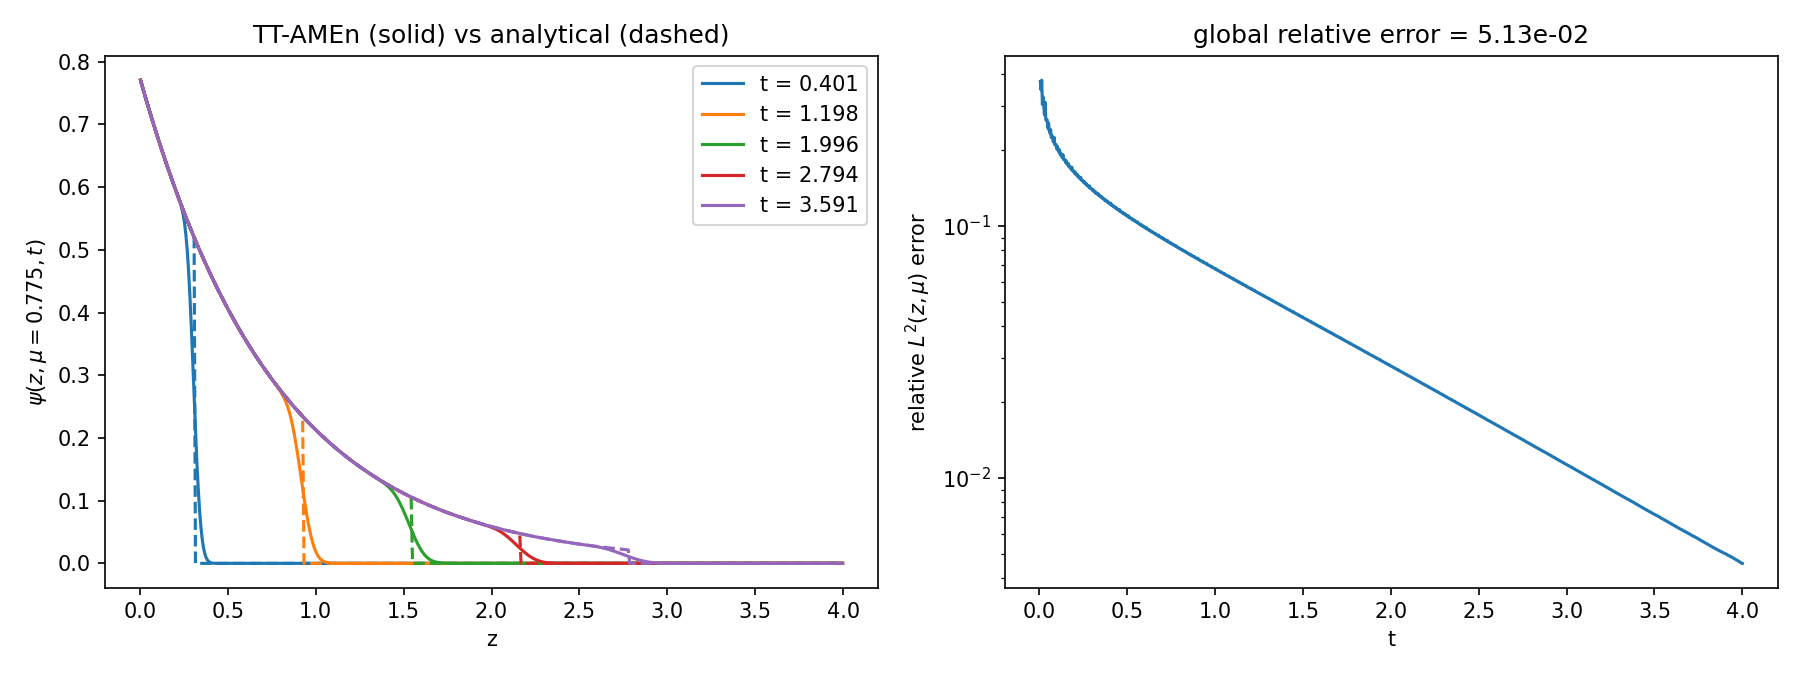
\includegraphics[width=\textwidth]{beam_front.png}
\caption{Beam entering a purely absorbing slab: zero source and initial condition. The front at $z=\mu vt$ is a discontinuity, which the scheme smears over several cells (numerical diffusion of the upwind DG / backward Euler scheme), giving a global relative error of $5\times10^{-2}$ that decreases in time as the front leaves the slab. This is the hardest test for the TT format: ranks reach 61 (compression only $\approx0.07$).}
\label{fig:beam_front}
\end{figure}

\begin{figure}[h!]
\centering
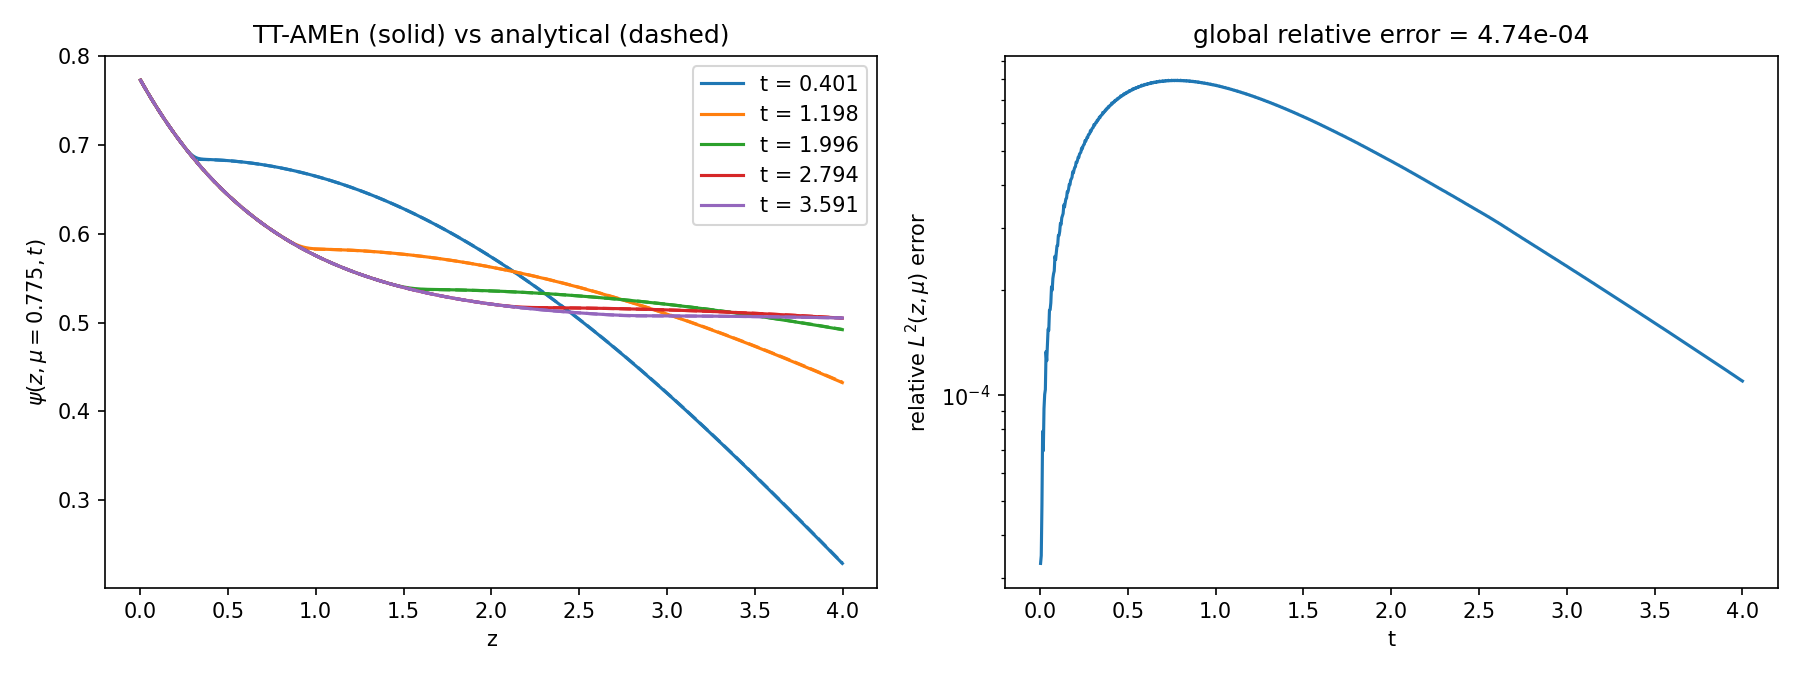
\includegraphics[width=\textwidth]{beam_source_ic.png}
\caption{Same slab with a constant isotropic source $Q=0.5$ and initial condition $\psi^{\mathrm{init}}=|\mu|\cos(\pi z/2L)$, chosen compatible with the inflow at the corner $(z,t)=(0,0)$ and with the zero right inflow. The solution is continuous (only its derivative jumps at $z=\mu vt$) and the global relative error drops to $5\times10^{-4}$.}
\label{fig:beam_source_ic}
\end{figure}

\FloatBarrier
\subsection{Infinite medium with isotropic scattering}
\label{sec:infinite}

Consider one group, isotropic scattering and $z\in\R$; only an initial condition $\psi_{\mathrm{IC}}$ is needed. Measuring lengths in mean free paths ($\sigma_tz\to z$) and time in collision times ($v\sigma_tt\to t$),
\begin{equation}
\Big(\pderiv{}{t}+\mu\pderiv{}{z}+1\Big)\psi(z,\Om,t)=\frac{c}{4\pi}\phi(z,t)+q(z,\Om,t),
\qquad\phi=\int_{4\pi}\psi\,\dd\Om,
\end{equation}
with scattering ratio $c=\sigma_s/\sigma_t$ and $q=Q/\sigma_t$.
With the Laplace transform in $t$ ($t\to s$) and the Fourier transform in $z$ ($z\to k$, $\partial_z\to ik$), denoted by a hat,
\begin{equation}
\hat\psi(k,\Om,s)=\frac{\hat\psi_{\mathrm{IC}}(k,\Om)+\frac{c}{4\pi}\hat\phi(k,s)+\hat q(k,\Om,s)}{s+1+ik\mu}.
\end{equation}
Integrating over $\Om$,
\begin{equation}
\hat\phi(k,s)=\frac{\hat q_0(k,s)+\hat\phi_{\mathrm{IC}}(k,s)}{1-\frac{c}{4\pi}T(k,s)},\qquad
T(k,s)=\int_{4\pi}\frac{\dd\Om}{s+1+ik\mu}=\frac{4\pi}{k}\arctan\frac{k}{s+1},
\label{eq:phi-hat}
\end{equation}
where $\hat q_0=\int_{4\pi}\frac{\hat q}{s+1+ik\mu}\dd\Om$ and $\hat\phi_{\mathrm{IC}}=\int_{4\pi}\frac{\hat\psi_{\mathrm{IC}}}{s+1+ik\mu}\dd\Om$. (The arctangent follows from $\int_{-1}^1\frac{\dd\mu}{a+ik\mu}=\int_{-1}^1\frac{a\,\dd\mu}{a^2+k^2\mu^2}=\frac2k\arctan\frac ka$. \cite{TransportTheory}) \Cref{eq:phi-hat} is inverted numerically following Ganapol \cite{AnBenchmarks} (\cref{app:inversion}).

\paragraph{Decaying Gaussian source, zero initial condition.}
For $q(z,\Om,t)=e^{-\alpha z^2}e^{-\lambda t}$ and $\psi_{\mathrm{IC}}=0$,
\begin{equation}
\hat q(k,s)=\sqrt{\frac\pi\alpha}\,\frac{e^{-k^2/4\alpha}}{s+\lambda},\qquad \hat q_0=\hat q\,T,\qquad
\hat\phi(k,s)=\sqrt{\frac\pi\alpha}\,\frac{e^{-k^2/4\alpha}}{s+\lambda}\,\frac{4\pi\arctan\big(k/(s+1)\big)}{k-c\arctan\big(k/(s+1)\big)}.
\end{equation}
The rightmost singularity is at $s=c-1$ (the $k\to0$ limit of the denominator), which fixes the Bromwich abscissa. In the TT solver the infinite medium is approximated by a slab of width $L=10$ with the Gaussian centred at $L/2$ and vacuum boundaries; for $T=1$ the boundaries are far enough that their influence is negligible.

\begin{figure}[h!]
\centering
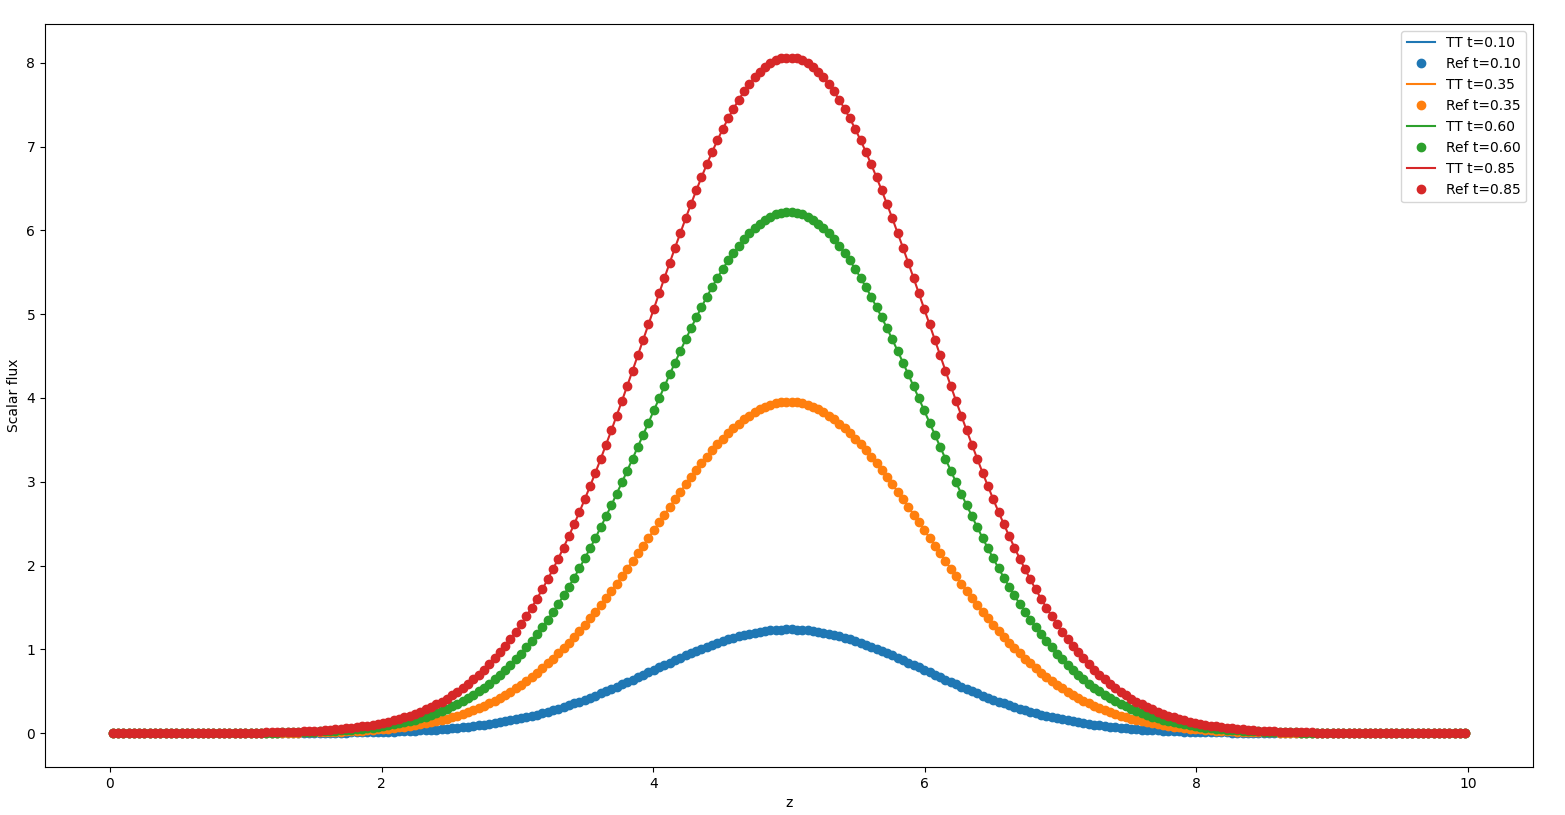
\includegraphics[width=0.8\textwidth]{decaying_gaussian_response.png}
\caption{Scalar flux for the decaying Gaussian source ($\alpha=0.5$, $\lambda=0.1$, $c=0.5$): TT solution versus the semi-analytical reference obtained by double numerical inversion (\cref{app:inversion}). Max relative $L^2$ error $\approx10^{-4}$. AMEn converges to a residual $\approx10^{-6}$ in $\approx20$ sweeps, max rank 13, compression $\approx10^{-5}$.}
\label{fig:decaying_gaussian_response}
\end{figure}

%==========================================================================================
\appendix
\section{Numerical inversion of integral transforms}
\label{app:inversion}
%==========================================================================================

\subsection{Inverse Fourier transform}

Convention: $F(k)=\int f(x)e^{-ik\cdot x}\,\dd^dx$, $f(x)=\int F(k)e^{ik\cdot x}\,\frac{\dd^dk}{(2\pi)^d}$.

\paragraph{One dimension.}
For real $f$, $F(-k)=\overline{F(k)}$ and
\begin{equation}
f(x)=\frac1\pi\int_0^\infty\big(\mathrm{Re}F(k)\cos kx-\mathrm{Im}F(k)\sin kx\big)\,\dd k .
\end{equation}
Following Ganapol \cite{AnBenchmarks} (see also \cite{IntegralTransforms}), substitute $u=k|x|$ and split $[0,\infty)$ into intervals of length $\pi$; since $\cos$ and $\sin$ change sign on consecutive intervals,
\begin{equation}
f(x)=\frac{1}{\pi|x|}\sum_{j=0}^{\infty}(-1)^j\int_0^\pi\Big(\mathrm{Re}F(k_j)\cos u-\sgn(x)\,\mathrm{Im}F(k_j)\sin u\Big)\dd u,
\qquad k_j=\frac{u+j\pi}{|x|}.
\end{equation}
The alternating series is summed with convergence acceleration. For $|x|<0.1$ the first interval is very long in $k$, so the first term is computed directly as $\frac1\pi\int_0^{\pi/|x|}(\dots)\,\dd k$ to avoid oscillations; at $x=0$ one uses $f(0)=\frac1\pi\int_0^\infty\mathrm{Re}F(k)\,\dd k$ with Gauss--Laguerre quadrature.
Observed relative errors: $\approx10^{-15}$ for smooth functions, $\approx10^{-4}$ for a rectangular pulse.

\paragraph{Two dimensions.}
In polar coordinates $(x,y)\to(r,\theta)$, $(k_x,k_y)\to(k,\phi)$ \cite{FourierTransforms},
\begin{equation}
f(r,\theta)=\frac{1}{(2\pi)^2}\int_0^{2\pi}\!\!\dd\phi\int_0^\infty F(k,\phi)\,e^{ikr\cos(\theta-\phi)}\,k\,\dd k .
\end{equation}
With the Jacobi--Anger expansion $e^{iz\cos\vartheta}=\sum_ni^nJ_n(z)e^{in\vartheta}$ and $F(k,\phi)=\sum_mF_m(k)e^{im\phi}$, $F_m=\frac1{2\pi}\int_0^{2\pi}F e^{-im\phi}\dd\phi$, the $\phi$-integral selects $m=n$:
\begin{equation}
f(r,\theta)=\frac{1}{2\pi}\sum_{n}i^ne^{in\theta}\int_0^\infty F_n(k)J_n(kr)\,k\,\dd k,
\qquad\text{radial case: } f(r)=\frac{1}{2\pi}\int_0^\infty F(k)J_0(kr)\,k\,\dd k .
\end{equation}
The Hankel integral can be computed with Ogata's quadrature (requires the substitution $x=kr$, which caused problems) or with adaptive quadrature (MATLAB \texttt{integral}), which behaves poorly when the integrand decays slowly.

\paragraph{Three dimensions.}
In spherical coordinates $x=r\Gamma$, $k=k\Om$,
\begin{equation}
f(r,\Gamma)=\frac{1}{(2\pi)^3}\int_{\mathbb{S}^2}\dd\Om\int_0^\infty F(k,\Om)\,e^{ikr\,\Gamma\cdot\Om}\,k^2\,\dd k .
\end{equation}
With $e^{ikr\Gamma\cdot\Om}=4\pi\sum_{l,m}i^lj_l(kr)\,\overline{Y_{lm}(\Om)}\,Y_{lm}(\Gamma)$ and $F(k,\Om)=\sum_{l,m}F_{lm}(k)Y_{lm}(\Om)$,
\begin{gather}
f(r,\Gamma)=\frac{1}{2\pi^2}\sum_{l,m}i^lY_{lm}(\Gamma)\int_0^\infty F_{lm}(k)\,j_l(kr)\,k^2\,\dd k,
\\\text{radial case: } f(r)=\frac{1}{2\pi^2}\int_0^\infty F(k)\,j_0(kr)\,k^2\,\dd k .
\end{gather}

\subsection{Inverse Laplace transform}

$f(t)=\frac{1}{2\pi i}\int_{\beta-i\infty}^{\beta+i\infty}F(s)e^{st}\,\dd s$, with $\beta$ to the right of all singularities of $F$.

\paragraph{Talbot's method. (not used in the code)}
Talbot \cite{Talbot} deforms the Bromwich line into a contour that wraps around the negative real axis,
\begin{equation}
s(\theta)=\beta+\varrho\,(\theta\cot\theta+i\nu\theta),\qquad-\pi<\theta<\pi,
\end{equation}
with tunable $\varrho,\nu>0$, so that
$f(t)=\frac{1}{2\pi i}\int_{-\pi}^{\pi}F(s(\theta))e^{s(\theta)t}s'(\theta)\,\dd\theta$,
which the trapezoidal rule integrates with spectral accuracy.

\paragraph{Fourier cosine series method.}
For real $f$ and $s=\beta+i\omega$ \cite{LaplInverse},
\begin{equation}
\mathrm{Re}F(\beta+i\omega)=\int_0^\infty e^{-\beta t}f(t)\cos\omega t\,\dd t
\quad\Longrightarrow\quad
f(t)=\frac{2e^{\beta t}}{\pi}\int_0^\infty\mathrm{Re}F(\beta+i\omega)\cos\omega t\,\dd\omega .
\end{equation}
Following \cite{AnBenchmarks}, substitute $\omega\to\omega/t$ and split into half-periods of the cosine:
\begin{equation}
f(t)=\frac{2e^{\beta t}}{\pi t}\left[\int_0^{\pi/2}\mathrm{Re}F\Big(\beta+\frac{i\omega}{t}\Big)\cos\omega\,\dd\omega
+\sum_{j=1}^\infty(-1)^j\int_{-\pi/2}^{\pi/2}\mathrm{Re}F\Big(\beta+\frac{i(\omega+j\pi)}{t}\Big)\cos\omega\,\dd\omega\right],
\end{equation}
and the alternating series is accelerated with the Euler--Knopp transform. For the Gaussian source of \cref{sec:infinite} the double (Fourier + Laplace) inversion reproduces $q(x,t)$ with relative error $\approx10^{-5}$ at all times.

%==========================================================================================
\section{Notation and code}
\label{app:code}
%==========================================================================================

\begin{center}\small
\renewcommand{\arraystretch}{1.2}
\begin{tabular}{@{}lll@{}}
\toprule
Symbol & Code (\texttt{SlabTransportModel}) & Notes \\
\midrule
$N_z,\ p,\ L,\ h$ & \texttt{N\_z, p, L\_z, h} & $N_s=N_z(p+1)=$ \texttt{ndof\_z} \\
$N_\mu,\ N_\varphi,\ G,\ N_t,\ T,\ \Delta t$ & \texttt{N\_mu, N\_phi, G, N\_t, T, dt} & $t_k=k\Delta t$, \texttt{t} \\
$\mu_n,w_n$;\ $\varphi_q,w_q$ & \texttt{mu, w\_mu; phi, w\_phi} & \\
$\mu_n^{+},\ \mu_n^{-}$ & \texttt{mu\_plus, mu\_minus} & \\
$M$ & \texttt{M} & global, $I_{N_z}\kron M_h$ \\
$S$ & \texttt{S} & local; $\mathsf S=I_{N_z}\kron S$ built inline \\
$\pp\pp^{\!\top},\ \pmn\pp^{\!\top},\ \pp\pmn^{\!\top},\ \pmn\pmn^{\!\top}$ & \texttt{B\_p\_R, B\_p\_L, B\_m\_R, B\_m\_L} & \\
$U^{+},\ U^{-}$ & \texttt{space} (``face terms'') & \\
$K$ & \texttt{K = heneey\_greenstein(...)} & \\
$\gamma,\ \Lmax$ & \texttt{gamma, L\_max} & \\
$E_g,\ v_g,\ v_0,\ E_{\max}$ & \texttt{E, v, v0, E\_max} & \\
$\sigma_{t,g}$,\ $C$ & \texttt{sigma\_t, C} & \texttt{C[g, g']}: $g'\to g$ \\
$s_a,\ \eta$ & \texttt{sigma\_a\_frac, eta} & \\
$\mathcal{A},\ F$ & \texttt{A, F} & \\
$F_Q,F_{\mathrm{init}},F_{\mathrm{left}},F_{\mathrm{right}}$ & \texttt{q, IC, BC\_L, BC\_R} & \\
$\Psi$ & \texttt{psi\_modal} (\texttt{psi}: at Gauss points) & \\
\bottomrule
\end{tabular}
\end{center}

\bibliographystyle{plain}
\bibliography{references}

\end{document}
